%% Given in Seattle, at the National Research Center for Statistics
%% and the Environment, and at MathSoft, October 1997.

\documentclass[semhelv]{seminar}
%% comment out the above and use below, if you have font troubles
%%\documentclass[semlcmss]{seminar}
%%\documentclass{seminar}

\usepackage{slidesec}
\usepackage[dvips]{graphicx}
%\usepackage{html,heqn,htmllist} % LaTeX2HTML support

\begin{document}

\typeout{ }
\typeout{If you have font troubles, comment out line 5 and
  uncomment line 7}
\typeout{ }

\begin{slide}
  \slideheading{ESS and Literate Programming: \\
    Tools for Efficient Statistical Programming and Data Analysis}

  \begin{center}
    Dr. A.J. Rossini \\
    Statistics Department \\
    University of South Carolina \\
    rossini@stat.sc.edu \\
 %   \htmladdnormallink{http://www.stat.sc.edu/\~{}rossini/rsrch/seattle-nrcse/}
%    {http://www.stat.sc.edu/\~{}rossini/rsrch/seattle-nrcse/} 
  \end{center}
  
  Note: \textbf{ESS} is joint work with: Martin Maechler (ETHZ), Kurt
  Hornik (TU-Wien), and Richard M. Heiberger (Temple).
\end{slide}

\begin{itemize}
\item Thanks also to Bates, Kademan, Ritter (initial versions), and
  David Smith (3.x, 4.x).
\end{itemize}

Recently, I've been giving talks which focus on Computer/Statistician
interfaces, like this one.  They tend to get strange responses.  This
is not too different from the applied/theoretical Comp Sci situation,
where journals focus both on software practice, as well as on theory.
Practitioners from both groups are also very confused.

So for today, we will focus on one area of statistical practice, as
opposed to statistical theory (methods/mathematics/data analysis).

\begin{slide}
  \slideheading{Introduction}
  
  Topics:
  \begin{itemize}
  \item Computing Environments
  \item ESS (=\emph{EMACS Speaks Statistics}), and its capabilities
  \item Literate Programming and Literate Data Analysis
  \item Links between ESS and Lit Prog
  \item Future (planned?) Extensions
  \end{itemize}

\end{slide}

\begin{itemize}
\item Outline of Talk
\end{itemize}

\begin{slide}
  \slideheading{Computing Environments}
  
  Computer / Statistician Interface:
  \begin{itemize}
  \item Command line: keyboard based, minimal mouse usage (SAS (old
    style), S-PLUS 3.x, R, XLispStat, Minitab (old style))
  \item Graphical: pointer (mouse)-based, ``point and click'', minimal
    keyboard usage (S-PLUS 4, ViSta, Minitab)
  \item Mixed Interfaces: S-PLUS 4, SAS, ViSta, Minitab
  \end{itemize}
  
  The \emph{Interface} is dependent on the particular user's practice
  (note the repetition of packages).
\end{slide}


\begin{itemize}
\item Importance to Statisticians. 
\item Issues of efficiency
\end{itemize}

\begin{slide}
  \slideheading{Computing Environments: Design Considerations}
  
  \begin{itemize}
  \item keyboard entry is faster than mouse entry (eventually?)
  \item mouse entry is easier than keyboard entry (initially?)
  \item At present, keyboard interfaces allow for more
    complex/powerful methods, but this is more a function of current
    software than a design limitation.
  \item Keyboard interfaces generally require memorization of some
    commands (at the minimum: those required to find others!).
  \end{itemize}
\end{slide}

\begin{itemize}
\item Not discussing using keyboard as a substitute for a
  mouse/pointer-based interface!  (i.e. keys to move the pointer, and
  to press the pointer buttons).
\end{itemize}

\begin{slide}
  \slideheading{Emacs}

  \begin{itemize}
  \item Text Editor (not a word processor)
  \item Fully Configurable and Extensible:
    \begin{itemize}
    \item Communication with system processes
    \item Automation of procedures (version control, file comparison)
    \item Language-specific customizations
  \end{itemize}
\end{itemize}

  Currently, comes in 2 GNU Flavors:
  \begin{itemize}
  \item Emacs (FSF/RMS developed)
  \item XEmacs (derivative of the above, more features, more bloat)
  \end{itemize}
  
\end{slide}

Some current modes:
\begin{itemize}
\item \LaTeX
\item C, Fortran, SQL
\item Makefiles
\item version control
\end{itemize}

XEmacs features:
\begin{itemize}
\item Embeddable images
\item mixed fonts and rich-text (near-WYSIWYG LaTeX document
  construction)
\end{itemize}

\begin{slide}
  \slideheading{ESS (=\emph{EMACS Speaks Statistics})}
  
  A package for Emacs, with the following features:
  \begin{itemize}
  \item Mode for generating program code for statistical packages
  \item Inclusion of statistical processes as inferior processes
    controlled through Emacs.
  \item Interface for on-line help features for statistical packages
    (via calls to the package, standard WWW documentation, etc)
  \item Interface for generating, documenting, and reusing transcripts
    for data analysis and development sessions.
  \end{itemize}

\end{slide}

\begin{itemize}
\item Discuss the README
\item What are we trying to do
\end{itemize}

\begin{slide}
  \slideheading{ESS capabilities: programming}

  \begin{itemize}
  \item Syntax-based color and font highlighting
  \item Access to on-line help facilities when inferior statistical
    processes are running; to WWW based facilities when not.
  \item Connection to statistical processes, ability to switch
    processes (i.e. different instantiations of the same dialect,
    different dialects)
  \end{itemize}
\end{slide}

\begin{itemize}
\item to improve code readability.
\item on-line help, split off into a different buffer.
\item connection to different processes:
  \begin{itemize}
  \item to compare different results
  \item to get different help information
  \end{itemize}
\end{itemize}


\begin{slide}
  \slideheading{ESS capabilities: inferior process}

  \begin{itemize}
  \item Syntax-based color and font highlighting
  \item Searchable Command History
  \item Separate buffers for help output
  \item Log (Transcript) of commands
  \item Debugging assistance (of source)
  \end{itemize}
\end{slide}

\begin{itemize}
\item to improve code readability.
\item ``Splus -e'' improved.
\item split up output by context (help, etc).
\end{itemize}

\begin{slide}
  \slideheading{ESS capabilities: transcript}

  \begin{itemize}
  \item Reuse of transcripts in different dialects, for different
    sessions. 
  \item Commenting of transcripts
  \item Comparison of output
  \end{itemize}
\end{slide}

\begin{itemize}
\item One use: authors who are targeting a number of dialects of S,
  S-PLUS, and R.
\item Readability
\item comparison of output among different statistical packages.
\end{itemize}

%\begin{slide}
%  \slideheading{ESS: examples}
  
%  %%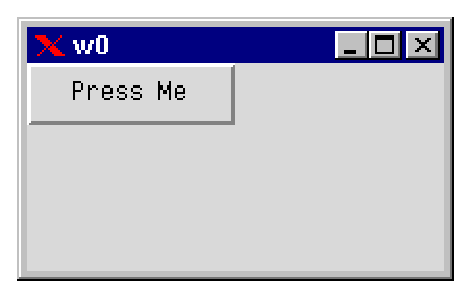
\includegraphics[height=3\semin,width=3\semin]{ex1.ps}

%  %%\includegraphics[height=3\semin,width=3\semin]{ex2.ps}

%\end{slide}

%Discuss example screen shots.

\begin{slide}
  \slideheading{ESS: future plans}

  \begin{itemize}
  \item Improved support for current languages
  \item Additional support for other languages (Fiasco/SPSS)
  \item Inlined statistical graphics (XEmacs)
  \item Object browser (partial implementation exists for SAS,
    eventually for S and XLispStat languages).
  \item Language independent UI/GUI for data analysis.
  \item Language independent UI/GUI for statistical instruction.
  \end{itemize}
\end{slide}

\begin{itemize}
\item ESS as a general purpose statistical GUI
\item ESS as a general purpose statistical instruction/assistance tool 
  \begin{itemize}
  \item Statistical help via WWW
  \item Download similar Analyses
  \item Guidance via Literate Data analysis
  \end{itemize}
\end{itemize}


\begin{slide}
  \slideheading{Why bother?}

  \begin{itemize}
  \item No real need to have a unifying mode (both too much and too
    little). 
  \item Different languages have different syntax
  \end{itemize}
  \textbf{BUT:}
  \begin{itemize}
  \item Common, generic interface.
  \item Improved documentation is important.
  \item To this goal, want to encourage documentation and revision
    logs:
    \begin{itemize}
    \item Revision and Source Control Systems (not discussed: SCCS,
      RCS, CVS, PRCS) (automated via Emacs, or manually implemented)
    \item Literate Programming (discussed)
    \end{itemize}
  \end{itemize}
\end{slide}

\begin{itemize}
\item Why 2 topics?
\item Single common mode for Literate Programming, Literate Data
  Analysis.
\item Revision/Source control is extremely useful for keeping track of
  document and program changes.  But will not be discussed today.
\end{itemize}

\begin{slide}
  \slideheading{Literate Programming: Introduction}

  \begin{itemize}
  \item Introduced by D.E.Knuth for developing \TeX (1984)
  \item Intent: The task of programming should shift from telling a
    computer what to do, to explaining to human beings what we are
    doing.
  \item Remark: Every use of the word \textbf{programming} (used
    before and after this) can be exchanged for the words \textbf{data
      analysis}.
  \end{itemize}
\end{slide}

\begin{itemize}
\item Origin
\item Goal: a means to document results.
\item \emph{Data Analysis} can be thought of as the implementation of
  a particular type/style of \emph{Programming}.
\end{itemize}

\begin{slide}
  \slideheading{Lit Prog: Example}
{\tiny
\begin{verbatim}
\section{Introduction}\label{intro}

For regression models with interval-censored data, there is generally no simply means of
conditioning out the nuisance parameter.  This nuisance parameter is generally a function of the
baseline cumulative distribution function, such as $\Lambda(t)$, the cumulative hazard function, or
$\Phi(t) = F(t)/S(t)$, the odds function. 

However, with right-censored data under the proportional hazards model, we can condition out the
nuisance parameter.  This simplifies and speeds up the resulting estimation. 

The main body of code will be the simulation routine, given by 

<<bag.sim.S>>=
  bag.sim <- function(beta,N,nobs,numBSsamp)  {
    <<simulation routine.S>> ;
    <<report and summarize results.S>> ;
  }
@ %def bag.sim N nobs beta numBSsamp

This can be divided into dataset generation and analysis sections.

<<simulation routine.S>>=
  for (i in 1:N)  {
    <<Generate data set.S>> ;
    <<Analyse data set using imputation and bootstrap.S>> ;
  }
@ %def i
\end{verbatim}
}
\end{slide}

\begin{itemize}
\item Basic example of literate programming.
\item document chunks start with '@'.
\item program chunks start with '\verb$<<$'
\end{itemize}

\begin{slide}
  \slideheading{Web Processing}

  \begin{itemize}
  \item To get documentation: weave a web  (forms: tex, html, etc).
  \item To get the code: tangle a web
  \end{itemize}
  idea: don't want to read or change raw code (and discourage this!);
  documentation should tell you everything.
\end{slide}

\begin{itemize}
\item Not WWW...
\item basically text processing.
\end{itemize}

\begin{slide}
  \slideheading{Statistical Programming and Data Analysis}
  
  Is there a difference? 
\end{slide}

\begin{itemize}
\item Why literate programming is of interest for data analysis
  documentation. 
\item at the most, differences just in the intended use of the code.

\end{itemize}

\begin{slide}
  \slideheading{Requirements in a Literate Programming Tool}
  (for statisticians)

  Program:
  \begin{itemize}
  \item Language independence 
  \item Platform independence
  \end{itemize}

  Statistician:
  \begin{itemize}
  \item discipline
  \item interest
  \end{itemize}
\end{slide}

\begin{itemize}
\item Language independence (examples: S-PLUS, C, Fortran code mixed
  interchangeably).
\item Flexible and platform independent
\end{itemize}

\begin{slide}
  \slideheading{Relationship between ESS and Lit Prog}
  
  Good:
  \begin{itemize}
  \item Documentation (using AUC-TeX), ease of programmability
  \item Ability to test out real code (dump straight into a running
    process).
  \end{itemize}
  Bad:
  \begin{itemize}
  \item Not fully automated (yet!).
  \item learn yet another language (or meta-language).
  \end{itemize}
  
\end{slide}

lack of automation implies that one needs to access a command line to
actually produce results.
 
\begin{itemize}
\item Current Links
\end{itemize}

\begin{slide}
  \slideheading{Future Extensions: ESS/Lit Prog}

\end{slide}

\begin{itemize}
\item Templates
\item Software packaging
\end{itemize}

\begin{slide}
  \slideheading{Where to find}

  \begin{itemize}
  \item ESS: http://ess.stat.wisc.edu/
    %%\htmladdnormallink{ESS} {http://www.stat.sc.edu/~rossini/projects/}:
  \item Literate Programming:
    \begin{itemize}
    \item General Information:
      http://www.desy.de/ftp/pub/userwww/projects/LitProg.html 
      %%\htmladdnormallink{General Information} {http://www.desy.de/ftp/pub/userwww/projects/LitProg.html} 
      %%\htmladdnormallink{http://www.desy.de/ftp/pub/userwww/projects/LitProg.html} {http://www.desy.de/ftp/pub/userwww/projects/LitProg.html}
    \item %%\htmladdnormallink{Frequently Asked Questions about Lit
      %%Prog}{http://shelob.ce.ttu.edu/daves/faq.html}:
      Frequently Asked Questions about Lit Prog: http://shelob.ce.ttu.edu/daves/faq.html
      %%\htmladdnormallink{http://shelob.ce.ttu.edu/daves/faq.html}  {http://shelob.ce.ttu.edu/daves/faq.html}
    \item %% \htmladdnormallink{Noweb} {http://www.cs.virginia.edu/~nr/noweb/intro.html}:
      %%\htmladdnormallink{http://www.cs.virginia.edu/~nr/noweb/intro.html}      {http://www.cs.virginia.edu/~nr/noweb/intro.html}
      Noweb: http://www.cs.virginia.edu/~nr/noweb/intro.html
    \end{itemize}
  \end{itemize}
\end{slide}

\begin{itemize}
\item Where to get it.
\end{itemize}

\end{document}
